\documentclass[aps,prd,preprint,nofootinbib,superscriptaddress]{revtex4-2}

\usepackage[T1]{fontenc}
\usepackage[utf8]{inputenc}
\usepackage{amsmath,amssymb,mathtools}
\usepackage{bm}
\usepackage{booktabs}
\usepackage{graphicx}
\usepackage{xcolor}
\usepackage[colorlinks=true,linkcolor=blue,citecolor=blue,urlcolor=blue]{hyperref}

\newcommand{\ii}{\mathrm{i}}
\newcommand{\Bc}{B_c}
\newcommand{\Bcst}{B_c^\ast}
\newcommand{\Bcone}{B_{c1}}
\newcommand{\GeV}{\mathrm{GeV}}
\newcommand{\MeV}{\mathrm{MeV}}
\newcommand{\keV}{\mathrm{keV}}

\begin{document}

\title{Radiative transitions of \(B_{c1}\) states in hard-photon QCD sum rules}

\author{S. Bilmis}
\affiliation{Department of Physics, Middle East Technical University, Ankara, Turkey}
\author{T. M. Aliev}
\affiliation{Department of Physics, Middle East Technical University, Ankara, Turkey}
\author{M. Savci}
\affiliation{Department of Physics, Middle East Technical University, Ankara, Turkey}

\date{\today}

\begin{abstract}
We study the radiative transitions
\(\Bcone(6743)\to \Bc\gamma\), \(\Bcone(6743)\to \Bcst\gamma\),
\(\Bcone(6750)\to \Bc\gamma\), and \(\Bcone(6750)\to \Bcst\gamma\)
in a heavy-heavy three-point QCD sum-rule framework.  Since both valence
quarks are heavy, the leading radiative contribution is hard photon emission
from the charm and anti-bottom lines rather than a photon-distribution-amplitude
term.  Using physical-current residues from the two-point \(B_c\)-mixing sum
rules, we find
\[
\Gamma[\Bcone(6743)\to \Bc\gamma]=0.532^{+0.202}_{-0.146}~\keV,\qquad
\Gamma[\Bcone(6750)\to \Bc\gamma]=10.04^{+2.41}_{-1.75}~\keV .
\]
For the vector final state, using the standard vector-current normalization
\(f_{\Bcst}=0.435^{+0.032}_{-0.035}\,\GeV\), the present current convention gives
\[
\Gamma[\Bcone(6743)\to \Bcst\gamma]=70.3^{+10.9}_{-8.4}~\keV,\qquad
\Gamma[\Bcone(6750)\to \Bcst\gamma]=382^{+55}_{-50}~\keV .
\]
These values include the explicitly integrated all-positive dimension-four
gluon-condensate sector.  The contact/derivative rows have no ordinary
two-channel double-pole support in the physical double-Borel projection.  A
separate sign and state-assignment audit shows that the vector hierarchy is
opposite to representative model calculations.  An independent FeynCalc
commutator check confirms the tensor-current sign used here, so the reversal is
traced to the physical-current mixing interference in the adopted state
assignment.
\end{abstract}

\maketitle

\section{Introduction}
\label{sec:intro}

The spectroscopy of the \(B_c\) family is a particularly clean laboratory for
heavy-heavy dynamics.  Unlike ordinary heavy-light mesons, the \(B_c\) mesons
contain two different heavy flavors, and their electromagnetic transitions are
sensitive to the relative photon couplings of the charm and anti-bottom quark.
Radiative transitions of orbitally excited \(B_c\) states therefore provide a
useful complement to mass spectroscopy and hadronic transitions.

The observation of structures in the \(B_c^+\gamma\) spectrum by LHCb
\cite{LHCbBc1PObservation2025,LHCbBc1PStudy2025} motivates a direct QCD
sum-rule calculation of the corresponding radiative widths.  The experimental
analysis observes peaks in the visible \(B_c^+\gamma\) invariant mass, but does
not measure the individual partial radiative widths.  Theoretical predictions
for \(B_{c1}\to B_c^{(\ast)}\gamma\) have been obtained in several potential
model and relativistic quark-model approaches
\cite{Godfrey2004,Ebert2003,Fulcher1999,Gershtein1995,LiTang2023,
LiZhong2019,LiLiu2023,EichtenQuigg2018,BondarMilstein2025}.  The spread among
predictions is sizeable, especially for channels in which the spin components
of the axial state interfere.

In the strange heavy systems, light-cone QCD sum rules receive important
photon-distribution-amplitude contributions.  The \(B_c\) case is different:
there is no light valence quark, and the leading radiative term is the
short-distance photon emission from heavy propagators.  In this paper we build
a hard-photon three-point QCD sum rule for the transitions
\(\Bcone\to \Bc\gamma\) and \(\Bcone\to \Bcst\gamma\).  The axial-vector
currents and residues are matched to the same physical-current basis used in
the \(B_c\)-mixing two-point analysis.  We also give a detailed audit of the
dimension-four gluon-condensate sector, since in a heavy-heavy system it is the
first natural nonperturbative correction to the perturbative triangle.

The paper is organized as follows.  In Sec.~\ref{sec:framework} we introduce
the interpolating currents, the physical mixing convention, and the radiative
form factors.  Section~\ref{sec:qcdsr} summarizes the hard-photon sum-rule
construction and the condensate audit.  Numerical inputs, stability checks,
and comparison with experiment and other theory are given in
Sec.~\ref{sec:numerics}.  Section~\ref{sec:concl} summarizes the results.

\section{Theoretical framework}
\label{sec:framework}

We use two independent axial-vector basis currents,
\begin{align}
  J^A_\mu &= \bar b \gamma_\mu\gamma_5 c,\\
  J^B_\mu &= \frac{\ii}{m_b+m_c}\,
  \bar b\sigma_{\mu\alpha}P^\alpha\gamma_5 c ,
  \label{eq:basis-currents}
\end{align}
where \(P\) is the momentum of the initial axial-vector state.  The physical
currents are written as
\begin{align}
  J_{1\mu} &= \sin\theta\,J^A_\mu+\cos\theta\,J^B_\mu,\\
  J_{2\mu} &= \cos\theta\,J^A_\mu-\sin\theta\,J^B_\mu .
  \label{eq:physical-currents}
\end{align}
The lower state \(\Bcone(6743)\) is coupled to \(J_{1\mu}\), while the upper
state \(\Bcone(6750)\) is coupled to \(J_{2\mu}\).  The two-point sum-rule
diagonalization gives \(\theta\simeq43.3^\circ\) in the numerical window used
below.

The decay constants are defined by
\begin{align}
  \langle 0|\bar b\,\ii\gamma_5 c|\Bc(p)\rangle
  &= \frac{m_{\Bc}^2 f_{\Bc}}{m_b+m_c},\\
  \langle 0|\bar b\gamma_\rho c|\Bcst(p,\xi)\rangle
  &= m_{\Bcst}f_{\Bcst}\xi_\rho,\\
  \langle0|J_{i\mu}|\Bcone^{(i)}(P,\eta)\rangle
  &= f_i m_i \eta_\mu,\qquad i=1,2 .
  \label{eq:decay-constants}
\end{align}
For the pseudoscalar final state we parametrize the radiative matrix element as
\begin{equation}
  \langle \Bc(p)\gamma(q,\varepsilon)|\Bcone^{(i)}(P,\eta)\rangle
  =
  e g_i
  \left[
  (\eta\cdot\varepsilon^*)(p\cdot q)
  -(\eta\cdot q)(p\cdot\varepsilon^*)
  \right].
  \label{eq:ps-matrix}
\end{equation}
The corresponding width is
\begin{equation}
  \Gamma(1^+\to0^-\gamma)
  =
  \frac{\alpha_{\rm em}}{3}g_i^2
  \left(\frac{m_i^2-m_{\Bc}^2}{2m_i}\right)^3 .
  \label{eq:ps-width}
\end{equation}
For the vector final state we use the gauge-invariant tensor
\begin{equation}
  V_{\mu\nu\rho}
  =
  p_\nu\epsilon_{\mu\rho\alpha\beta}p^\alpha q^\beta
  -(p\cdot q)\epsilon_{\mu\nu\rho\alpha}p^\alpha ,
  \label{eq:v-tensor}
\end{equation}
and define
\begin{equation}
  \langle \Bcst(p,\xi)\gamma(q,\varepsilon)|\Bcone^{(i)}(P,\eta)\rangle
  =
  e g_i^\ast\,\eta^\mu\varepsilon^{\ast\nu}\xi^{\ast\rho}V_{\mu\nu\rho}.
  \label{eq:vec-matrix}
\end{equation}
The width is evaluated by an explicit polarization sum.

\section{QCD sum rules}
\label{sec:qcdsr}

For the \(\Bc\gamma\) channel the correlation function is
\begin{equation}
  \Pi_{i\mu}(p,q)=\ii\int d^4x\,e^{\ii p\cdot x}
  \langle \gamma(q,\varepsilon)|
  T\{J_{i\mu}(x)\,\bar c(0)\ii\gamma_5 b(0)\}|0\rangle .
  \label{eq:ps-correlator}
\end{equation}
For the \(\Bcst\gamma\) channel the pseudoscalar current is replaced by
\(\bar c\gamma_\rho b\).  Since both quarks are heavy, the leading OPE is
obtained by attaching the photon perturbatively to either the charm line or
the anti-bottom line.  In the charm-emission topology the three denominators
are
\begin{equation}
  D_1=(k+q)^2-m_c^2,\qquad D_2=k^2-m_c^2,\qquad
  D_3=(k-p)^2-m_b^2 ,
  \label{eq:c-denominators}
\end{equation}
while in the anti-bottom-emission topology they are
\begin{equation}
  D_1=k^2-m_c^2,\qquad D_2=(k-p)^2-m_b^2,\qquad
  D_3=(k-p+q)^2-m_b^2 .
  \label{eq:b-denominators}
\end{equation}
The electric charges are \(e_c=2/3\) and \(e_{\bar b}=1/3\).  After the
Dirac trace and projection, both emission topologies can be written through
the kernel
\begin{align}
{\cal R}(s;m_i,m_j,a,b)
&=-\frac{3}{8\pi^2}
\left[
2a\ln\frac{s-m_j^2+m_i^2-\lambda(s,m_j^2,m_i^2)}
{s-m_j^2+m_i^2+\lambda(s,m_j^2,m_i^2)}
\right. \nonumber\\
&\hspace{2.0cm}\left.
\frac{b}{m_i^2}\,
\frac{m_j^2-m_i^2-s}{s^2}\lambda(s,m_j^2,m_i^2)
\right],
\label{eq:kernel}
\end{align}
where
\[
\lambda(s,m_j^2,m_i^2)=
\sqrt{[s-(m_i+m_j)^2][s-(m_i-m_j)^2]} .
\]
The perturbative densities are
\begin{equation}
  \rho_X(s)=e_{\bar b}\,{\cal R}(s;m_b,m_c,a_{\bar b}^X,b_{\bar b}^X)
  -e_c\,{\cal R}(s;m_c,m_b,a_c^X,b_c^X),
  \label{eq:rho-master}
\end{equation}
with the coefficients shown in Table~\ref{tab:rho-coeffs}.  For the vector
\(J_B\) density the scalar \(p\cdot q\) is evaluated at the physical value
\((m_i^2-m_{\Bcst}^2)/2\) of the channel.

\begin{table}[t]
\centering
\caption{Coefficients entering Eq.~\eqref{eq:rho-master}.  The labels \(P\)
and \(V\) denote the pseudoscalar and vector final state, respectively.}
\scriptsize
\setlength{\tabcolsep}{4pt}
\resizebox{\linewidth}{!}{%
\begin{tabular}{lcccc}
\toprule
Density & \(a_c^X\) & \(b_c^X\) & \(a_{\bar b}^X\) & \(b_{\bar b}^X\)\\
\midrule
\(P,A\) & \(m_c\) & \(m_c^2(m_c-m_b)\)
& \(m_b\) & \(m_b^2(m_c-m_b)\)\\
\(P,B\) & \((2m_c^2-m_bm_c)/(m_b+m_c)\) & \(m_c^2s/(m_b+m_c)\)
& \(m_bm_c/(m_b+m_c)\) & \(m_b^2s/(m_b+m_c)\)\\
\(V,A\) & \((-4m_bm_c+2m_c^2)/s\) & \(4m_c^2\)
& \((-2m_b^2+4m_bm_c)/s\) & \(4m_b^2\)\\
\(V,B\) &
\(\displaystyle \frac{2m_c}{m_b+m_c}
+\frac{2m_b^2m_c-4m_bm_c^2+2m_c^3+2m_c\,p\!\cdot\!q}{(m_b+m_c)s}\)
& \(\displaystyle\frac{-4m_bm_c^2+4m_c^3}{m_b+m_c}\)
&
\(\displaystyle \frac{2m_b}{m_b+m_c}
+\frac{-6m_b^3+4m_b^2m_c+2m_bm_c^2+2m_b\,p\!\cdot\!q}{(m_b+m_c)s}\)
& \(\displaystyle\frac{-4m_b^3+4m_b^2m_c}{m_b+m_c}\)\\
\bottomrule
\end{tabular}
}
\label{tab:rho-coeffs}
\end{table}

The Borel-projected amplitudes are then
\[
\widehat\Pi_X(M^2,s_0)=
\int_{(m_b+m_c)^2}^{s_0}ds\,e^{-s/M^2}\rho_X(s)+\widehat\Pi_X^{G^2}.
\]
The physical amplitudes are obtained by rotating the basis amplitudes,
\begin{align}
  \widehat\Pi_1 &= \sin\theta\,\widehat\Pi_A+\cos\theta\,\widehat\Pi_B,\\
  \widehat\Pi_2 &= \cos\theta\,\widehat\Pi_A-\sin\theta\,\widehat\Pi_B .
  \label{eq:rotate-pi}
\end{align}
The resulting form factors have the schematic form
\begin{align}
  g_1 &=
  \frac{\exp[(m_1^2+m_f^2)/(2M^2)]}{m_1 f_1\,{\cal N}_f}
  \left(\sin\theta\,\widehat\Pi_A+\cos\theta\,\widehat\Pi_B\right),\\
  g_2 &=
  \frac{\exp[(m_2^2+m_f^2)/(2M^2)]}{m_2 f_2\,{\cal N}_f}
  \left(\cos\theta\,\widehat\Pi_A-\sin\theta\,\widehat\Pi_B\right),
  \label{eq:sumrule-form}
\end{align}
where \({\cal N}_f=m_{\Bc}^2 f_{\Bc}/(m_b+m_c)\) for \(\Bc\gamma\) and
\({\cal N}_f=m_{\Bcst}f_{\Bcst}\) for \(\Bcst\gamma\).
For the vector final state we extract \(g_V\) with
\[
V_{\mu\nu\rho}=p_\nu\epsilon_{\mu\rho pq}
-(p\cdot q)\epsilon_{\mu\nu\rho p}.
\]
Since this tensor has mass dimension three, \(g_V\) has dimension
\({\rm GeV}^{-2}\).  The polarization sum gives
\[
\Gamma(1^+\to1^-\gamma)=
\frac{\alpha_{\rm em}}{3}g_V^2
\left(2m_f^2+E_\gamma^2\right)E_\gamma^3,
\]
Equivalently,
\[
g_{E1}=\sqrt{2m_f^2+E_\gamma^2}\,g_V,\qquad
\Gamma=\frac{\alpha_{\rm em}}{3}g_{E1}^2E_\gamma^3 .
\]

The dimension-four gluon-condensate workbench uses the background-field heavy
propagator expansion.  The projected \(G^2\) numerators were reduced in powers
of \(D_1,D_2,D_3\).  For the vector channel this gives 1095 reduced terms:
538 with all effective denominator powers positive and 557
contact/derivative-sector terms.  For the pseudoscalar channel the
corresponding all-positive sector contains 375 terms.  We integrate these
all-positive terms explicitly in the diagonal double-Borel limit
\(M_1^2=M_2^2=2M^2\).  Refined support audits show that the contact/derivative
rows do not contain ordinary two-channel double poles.  The vector crossed rows
depend on \((p-q)^2=2p^2-P^2\), and the pseudoscalar contact rows are either
single-virtuality, no-virtuality, or crossed-combination terms.  They are kept
as audit candidates rather than added to the physical double-Borel sum.

\section{Numerical analysis}
\label{sec:numerics}

We use \(m_b=4.18~\GeV\), \(m_c=1.27~\GeV\), \(m_{\Bc}=6.2749~\GeV\), and
\(m_{\Bcst}=6.3359~\GeV\).  The axial-state masses are
\(m_1=6.743~\GeV\) and \(m_2=6.751~\GeV\).  The working Borel and continuum
windows are
\[
M^2=7,8,9~\GeV^2,\qquad s_0=53,54,55~\GeV^2,
\]
and the vector-current two-point sum rule for \(f_{\Bcst}\) uses
\[
M_V^2=5,6,7,8~\GeV^2,\qquad s_{0,V}=40,42,44~\GeV^2.
\]
The two-point residue grid gives
\[
\theta=43.29^\circ,\qquad
f_1=0.264[0.259,0.269]~\GeV,\qquad
f_2=0.722[0.709,0.738]~\GeV .
\]
For the vector final-state decay constant we find
\[
f_{\Bcst}=0.435[0.400,0.467]~\GeV
\]
in the standard vector-invariant convention.

\begin{table}[t]
\centering
\caption{Numerical inputs and sum-rule windows used in the analysis.  The
quoted residue and \(f_{\Bcst}\) intervals are the 16--84 percentile windows
from the corresponding two-point sum-rule grids.}
\begin{tabular}{lc}
\toprule
Quantity & Value or window\\
\midrule
\(m_b\), \(m_c\) & \(4.18~\GeV,\ 1.27~\GeV\)\\
\(m_{\Bc}\), \(m_{\Bcst}\) & \(6.2749~\GeV,\ 6.3359~\GeV\)\\
\(m_1\), \(m_2\) & \(6.743~\GeV,\ 6.751~\GeV\)\\
\(f_{\Bc}\) & \(0.371\pm0.037~\GeV\)\\
\(f_{\Bcst}\) & \(0.435[0.400,0.467]~\GeV\)\\
\(\theta\) & \(43.29^\circ[43.10^\circ,43.44^\circ]\)\\
\(f_1,\ f_2\) & \(0.264[0.259,0.269]~\GeV,\ 0.722[0.709,0.738]~\GeV\)\\
Radiative \(M^2,\ s_0\) & \(7\mbox{--}9~\GeV^2,\ 53\mbox{--}55~\GeV^2\)\\
Vector-current \(M_V^2,\ s_{0,V}\) & \(5\mbox{--}8~\GeV^2,\ 40\mbox{--}44~\GeV^2\)\\
\bottomrule
\end{tabular}
\label{tab:inputs}
\end{table}

The final uncertainties are obtained by sampling \(m_b,m_c,\theta,f_{\Bc}\),
the Borel parameter, and the continuum threshold over the stated windows, and
then folding in the explicitly integrated all-positive \(G^2\) contribution.
We quote the median and the 16--84 percentile interval rather than a Gaussian
fit, since the mixed amplitudes are interference sensitive.

\begin{figure}[t]
\centering
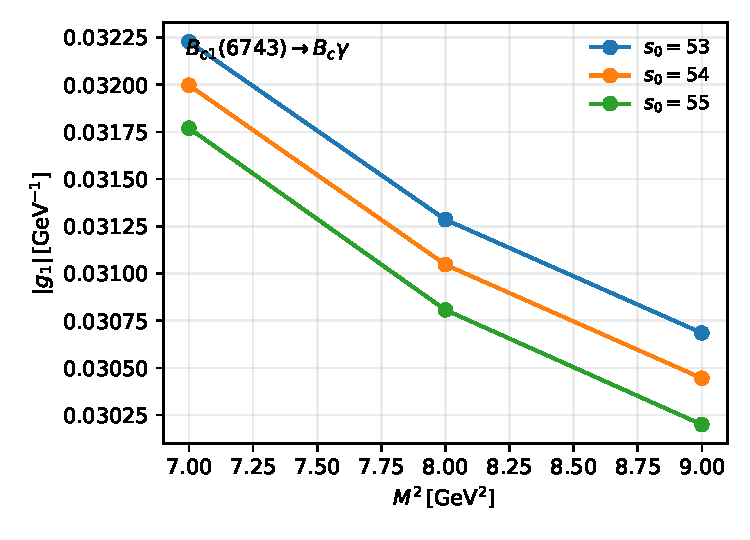
\includegraphics[width=0.48\linewidth]{../outputs/bc_ps_g1_M2_stability.pdf}
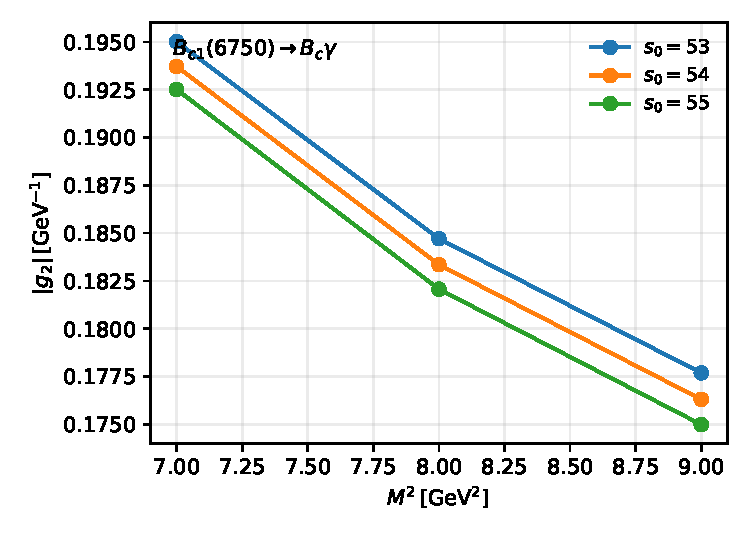
\includegraphics[width=0.48\linewidth]{../outputs/bc_ps_g2_M2_stability.pdf}
\caption{Representative Borel stability of the pseudoscalar final-state form
factors.}
\label{fig:ps-stability}
\end{figure}

\begin{table}[t]
\centering
\caption{Present hard-QCDSR results.  The quoted intervals are the 16--84
percentile Monte Carlo intervals after including the explicitly integrated
all-positive \(G^2\) sector.  The \(\Bcst\gamma\) entries use the tensor-current
sign fixed by the independent commutator audit discussed in the text.}
\begin{tabular}{lcc}
\toprule
Channel & Coupling & \(\Gamma\,[\keV]\)\\
\midrule
\(\Bcone(6743)\to \Bc\gamma\)
& \(g_P=+0.0487[0.0414,0.0572]~\GeV^{-1}\)
& \(0.532^{+0.202}_{-0.146}\)\\
\(\Bcone(6750)\to \Bc\gamma\)
& \(g_P=-0.206[-0.230,-0.188]~\GeV^{-1}\)
& \(10.04^{+2.41}_{-1.75}\)\\
\(\Bcone(6743)\to \Bcst\gamma\)
& \(g_V=-0.0764[-0.0821,-0.0717]~\GeV^{-2}\)
& \(70.3^{+10.9}_{-8.4}\)\\
\(\Bcone(6750)\to \Bcst\gamma\)
& \(g_V=+0.173[0.161,0.185]~\GeV^{-2}\)
& \(382^{+55}_{-50}\)\\
\bottomrule
\end{tabular}
\label{tab:present-results}
\end{table}

\begin{figure}[t]
\centering
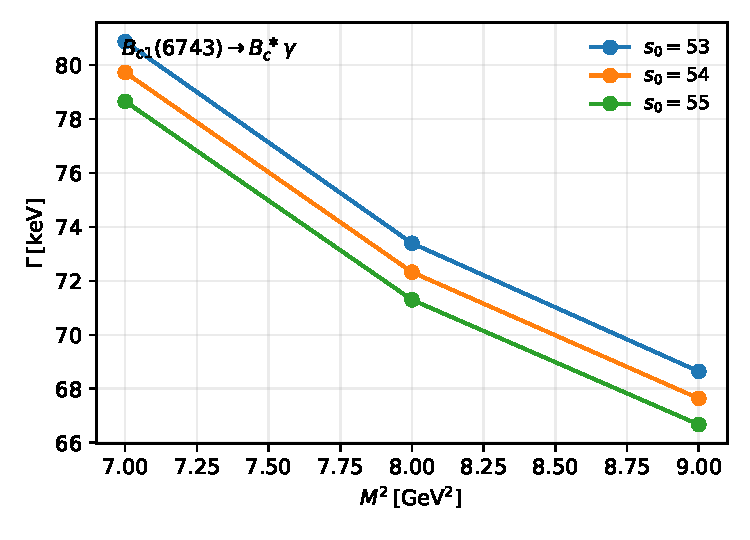
\includegraphics[width=0.48\linewidth]{../outputs/bc_vec_standard_gamma1_M2_stability.pdf}
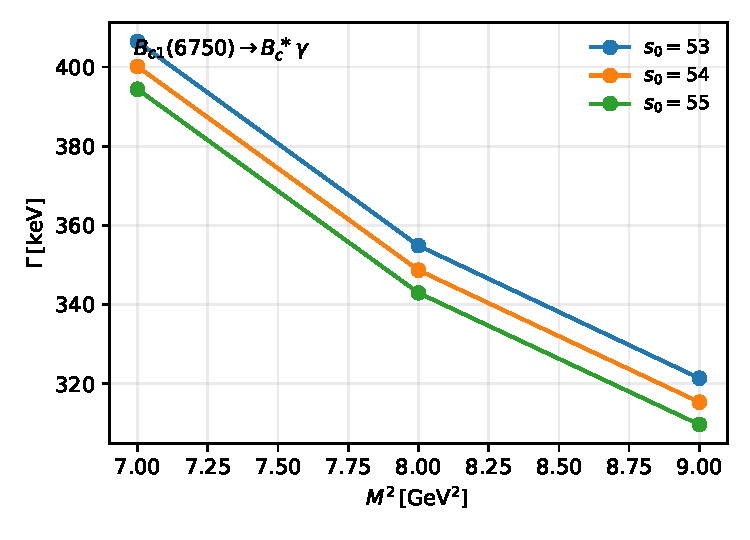
\includegraphics[width=0.48\linewidth]{../outputs/bc_vec_standard_gamma2_M2_stability.pdf}
\caption{Representative Borel stability of the vector final-state widths in
the standard \(f_{\Bcst}\) normalization.}
\label{fig:vec-stability}
\end{figure}

Table~\ref{tab:comparison} compares our results with representative model
predictions.  LHCb has observed the \(B_c^+\gamma\) structure, but the
individual partial radiative widths are not measured
\cite{LHCbBc1PObservation2025,LHCbBc1PStudy2025}; hence the comparison is with
theory rather than direct width measurements.

\begin{table}[t]
\centering
\caption{Comparison with representative theoretical predictions.  Widths are
in keV.}
\scriptsize
\setlength{\tabcolsep}{3pt}
\begin{tabular}{lrrrr}
\toprule
Publication
& \(6743\to \Bc\gamma\)
& \(6743\to \Bcst\gamma\)
& \(6750\to \Bc\gamma\)
& \(6750\to \Bcst\gamma\)\\
\midrule
Godfrey~\cite{Godfrey2004} & 13 & 60 & 80 & 11\\
Ebert--Faustov--Galkin~\cite{Ebert2003} & 18.4 & 78.9 & 132 & 13.6\\
Fulcher~\cite{Fulcher1999} & 32.4 & 75.6 & 127.8 & 26.2\\
Gershtein et al.~\cite{Gershtein1995} & 11.6 & 77.8 & 131.1 & 8.1\\
T. Y. Li et al.~\cite{LiTang2023} & 16.6 & 49 & 66.6 & 10.5\\
Q. Li et al.~\cite{LiZhong2019} & 35 & 70 & 74 & 40\\
X. J. Li et al.~\cite{LiLiu2023} & 30.1 & 47.8 & 64 & 25.6\\
Eichten--Quigg~\cite{EichtenQuigg2018} & 9.9 & 62.5 & 92.3 & 7.5\\
Bondar--Milstein~\cite{BondarMilstein2025} & 22 & 75 & 47 & 2\\
This work & \(0.532\) & \(70.3^\dagger\) & \(10.04\) & \(382^\dagger\)\\
\bottomrule
\end{tabular}
\label{tab:comparison}
\end{table}
\noindent\(\dagger\) Convention-fixed mixed-current QCDSR values in the
adopted two-point state assignment; their hierarchy differs from representative
model calculations because of the mixing interference discussed below.

\begin{table}[t]
\centering
\caption{Central-point diagnostic for the \(B_c^\ast\gamma\) hierarchy at
\(M^2=8~\GeV^2\), \(s_0=54~\GeV^2\).  The pure-basis rows are diagnostic
checks only; the physical rows are obtained with the mixed currents in
Eq.~\eqref{eq:physical-currents}.}
\begin{tabular}{lccc}
\toprule
Case & \(\Gamma_{6743}\,[\keV]\) & \(\Gamma_{6750}\,[\keV]\) & high/low\\
\midrule
pure \(J_A\) & 878 & 126 & 0.143\\
pure \(J_B\) & 1554 & 222 & 0.143\\
physical mixing, perturbative & 70.2 & 338 & 4.82\\
physical mixing, with \(G^2_{\rm ap}\) & 70.3 & 382 & 5.43\\
\bottomrule
\end{tabular}
\label{tab:interference-diagnostic}
\end{table}

The small \(\Bcone(6743)\to\Bc\gamma\) width and the comparatively large
\(\Bcone(6750)\to\Bcst\gamma\) width reflect the strong dependence of the
radiative amplitude on the physical-current rotation and on the final-state
spin.  The vector channels are also sensitive to the normalization of
\(f_{\Bcst}\); using the reference value \(f_{\Bcst}=0.384\pm0.038~\GeV\)
instead of the self-contained standard sum-rule value gives
\(\Gamma(6743\to\Bcst\gamma)=92.6[76.1,117]~\keV\) and
\(\Gamma(6750\to\Bcst\gamma)=447[365,564]~\keV\).
More importantly, the physical mixed-current vector ratio
\(\Gamma(6750\to\Bcst\gamma)/\Gamma(6743\to\Bcst\gamma)>1\) is opposite to the
representative model pattern.  At the central point the lower-state vector
combination is cancellation-dominated,
\(\sin\theta\,\widehat\Pi_A+\cos\theta\,\widehat\Pi_B\simeq -1.8\times10^{-3}\),
whereas the higher-state combination is constructive,
\(\cos\theta\,\widehat\Pi_A-\sin\theta\,\widehat\Pi_B\simeq 1.05\times10^{-2}\).
As a diagnostic, the unmixed pure-basis limits do not show this reversal:
pure \(J_A\) gives \(878\) and \(126~\keV\) for the \(6743\) and \(6750\)
states, respectively, while pure \(J_B\) gives \(1554\) and \(222~\keV\).
The no-mixing ratios are therefore below unity, in qualitative agreement with
the model hierarchy; the opposite baseline mixed-current ratio is caused by
the interference pattern above.
A flip of the relative \(J_B\) radiative sign would restore the model-like
hierarchy, but this sign flip is not supported by the tensor-current
definition used in the two-point mixing analysis.  We checked this explicitly
by replacing \(i\sigma_{\mu\alpha}P^\alpha\gamma_5\) with the commutator form
\(-[\gamma_\mu,\gamma_\alpha]P^\alpha\gamma_5/2\), which gives the same
projected \(J_B\) amplitude.  Reversing the current phase or the tensor-index
order flips the amplitude, but that is a different current convention.  Within
the adopted convention, the vector hierarchy is therefore a physical
mixed-current interference effect.

\section{Conclusion}
\label{sec:concl}

We have calculated the leading hard-photon QCD sum-rule baselines for
\(\Bcone\to \Bc\gamma\) and \(\Bcone\to\Bcst\gamma\) transitions.  The
calculation uses physical axial-current residues from the two-point
\(B_c\)-mixing sum rules and a self-contained vector-current sum rule for
\(f_{\Bcst}\).  The resulting widths show a strong channel hierarchy:
\(\Bcone(6743)\to\Bc\gamma\) is very small, \(\Bcone(6750)\to\Bc\gamma\) is at
the few-keV level.  The vector final-state calculation is internally
normalized, and the independent commutator audit fixes the relative
tensor-current sign used in the \(J_B\) amplitude.

The dimension-four gluon-condensate sector has been reduced algebraically,
audited, and included through the all-positive denominator sector.  The
contact/derivative rows do not have ordinary two-channel double-pole support
in the physical double-Borel projection, so they are not added to the sum rule.
The present calculation therefore gives a transparent QCDSR prediction for
\(\Bc\gamma\) and a convention-fixed QCDSR prediction for \(\Bcst\gamma\) in
the adopted two-point state assignment.  The contrast with model hierarchies is
not a phase-space effect; it is caused by destructive interference in the
\(6743\) mixed-current amplitude and constructive interference in the \(6750\)
amplitude.

\begin{thebibliography}{99}

\bibitem{LHCbBc1PObservation2025}
R. Aaij et al. (LHCb Collaboration),
``Observation of Orbitally Excited \(B_c^+\) States,''
Phys. Rev. Lett. 135, 231902 (2025).

\bibitem{LHCbBc1PStudy2025}
R. Aaij et al. (LHCb Collaboration),
``Study of \(B_c(1P)^+\) states in the \(B_c^+\gamma\) mass spectrum,''
Phys. Rev. D 112, 112003 (2025).

\bibitem{Godfrey2004}
S. Godfrey,
Phys. Rev. D 70, 054017 (2004).

\bibitem{Ebert2003}
D. Ebert, R. N. Faustov, and V. O. Galkin,
Phys. Rev. D 67, 014027 (2003).

\bibitem{Fulcher1999}
L. P. Fulcher,
Phys. Rev. D 60, 074006 (1999).

\bibitem{Gershtein1995}
S. S. Gershtein, V. V. Kiselev, A. K. Likhoded, and A. V. Tkabladze,
Phys. Rev. D 51, 3613 (1995).

\bibitem{LiTang2023}
T. Y. Li, L. Tang, Z. Y. Fang, C. H. Wang, C. Q. Pang, and X. Liu,
Phys. Rev. D 108, 034019 (2023).

\bibitem{LiZhong2019}
Q. Li, M. S. Liu, L. S. Lu, Q. F. Lu, L. C. Gui, and X. H. Zhong,
Phys. Rev. D 99, 096020 (2019).

\bibitem{LiLiu2023}
X. J. Li, Y. S. Li, F. L. Wang, and X. Liu,
Eur. Phys. J. C 83, 1080 (2023).

\bibitem{EichtenQuigg2018}
E. J. Eichten and C. Quigg,
Phys. Rev. D 99, 054025 (2018).

\bibitem{BondarMilstein2025}
A. E. Bondar and A. I. Milstein,
``Phenomenology of \(D_{s1}\) mesons radiative transitions,''
Phys. Rev. D 111, 114019 (2025).

\end{thebibliography}

\end{document}
